% !TeX root = ../main.tex

\chapter{The semi-classical (true) variational approach (WD)}

Starting from the two problems
\begin{center}
  \begin{minipage}{.48\linewidth}
    \centering
    \begin{tikzpicture}
      \draw (0,0) node [left] {$A$}
        to[bend right = 10] (2,-2) node [right] {$B$};
    \end{tikzpicture}
    \[
      \delta \int \d \tau = 0
    \]
  \end{minipage}
  \hspace* \fill
  \begin{minipage}{.48\linewidth}
    \centering
    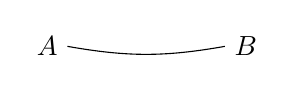
\begin{tikzpicture}
      \draw (0,0) node [left] {$A$}
        to[bend right = 10] (2,0) node [right] {$B$};
    \end{tikzpicture}
    \[
      \delta \int \d l F = 0
    \]
  \end{minipage}
\end{center}
We actually let $\delta \int \d \mathcal L = 0$, i.e., the Euler-Lagrangian EOM.
If it contains the interaction term, then we have the
\emph{Differential-intego-equation}

\section{Variational calculation for free fermions}

\[
  F[n(E)] = \tilde E[n(E)] - TS[n(E)] = \int \d E\phi(E,n)
\]
where $S = -n\ln n - (1 - n)\ln(1 - n)$.
The particle number conservation
\[
  N = \int \d E g(E) n(E), \quad \tilde E = \int \d E E n(E)
\]
We have to minimize the density function
\begin{equation}
  \fdv F{n(E)} \Rightarrow \pdv\phi n = \cdots \Rightarrow
  n^0(E) = \frac1{\upe^{(E-M)/T} + 1}
\end{equation}
also for $\fdv F\mu$.

\subsection{Generic variation around $n^0$}

The energy
\[
  E_0 = \int \frac{\d^ak}{(2\pi)^a} n_k^0 (\epsilon(k))
\]
where $\delta$ expanding some functional (function of functions)
\[
  \delta n_k(\epsilon(k)) = \nu^0(k)
+ \underbrace{\sum_{i = x_i} \pdv n{k_i}
  \bigg|_{n_k^1 \to n^0}}_{\delta(k - k)F,\ \text{The quasi-particle weight}}
  \nu_{k_i}^{(1)} + \frac12 \sum_{i,j} \pdv n{k_i,k_j}
  \underbrace{\nu_{k_ik_j}^{(2)}}_{\pdv n{k_i,k_j}}
\]
To the energy,
\[
  \delta E_0 = \delta \int \frac{\d k}{2\pi} n_k \epsilon_k
= \int \frac{\d k}{2\pi} \epsilon_k \delta n_k
\]
To put $\delta n_k$ into it,
\[
  \fdv En = \fdv*[fun]{\delta E_0 + V(\delta n_k)}n = 0
\]
Now, focus on $T = 0$, then $n_k^{(0)} = \Theta (\epsilon(k) - \mu)$,
$\epsilon_{k_F} - \mu = 0$
\[
  \pdv{n_k^{(0)}}k = \delta(\epsilon(k) - \mu)
  \pdif{k_i} \epsilon \big|_{k\to k_F}
\]
Then, the second derivative
\[
  \pdv{n^{(0)}}{k_i,k_j}
= \ab[\underbrace{\delta (\epsilon - \mu)}_{\delta(k_\bot - k_{F,\bot})}
    \pdif[2]{k_ik_j} \epsilon(k)   \big|_{k\to k_F}
    + \delta'(\epsilon - \mu) \pdif{k_i} \epsilon \pdif{k_j} \big|_{k\to k_F}]
\]
Note that $\delta(k_\bot - k_{F,\bot}) \neq \delta(k - k_r)$, since the shape of
the Fermi surface is arbitrary.
where we can spearate the motion around the Fermi surface into the
parallel and perpendicular terms.
In the simple case single connected Fermi surface
\[
  k_F(\theta) = (k_{r,F}(\theta) \cos\theta, k_{r,F}(\theta) \sin\theta)
\]
where $k_{r,F} (\theta) = k_{r,F_0} + k^0\cos\theta + \cdots$.

Now, we can build the connection between energy and 
\begin{multline}
  \delta E = \int \d \theta \d k_r k_r(\epsilon - \mu)
  (\nu^{(0)} + \delta(k_r - k_{r,F}(\theta)))
  (\pdif{k_r}\epsilon \nu_{k_r} + k_r^{-1} \pdif\theta\epsilon \nu_\theta\\
  + \frac12 \pdif[2]{k_r} \epsilon \nu_{k,k_r} + \cdots) + 
  \frac12\delta'(\epsilon(k) - \mu) (\qquad)
\end{multline}
where
\[
  \nu_{k_r} = \frac{\nu_{k_x}}{\cos\theta} + \frac{\nu_{k_y}}{\sin\theta}, \quad
  \nu_{k_\theta} = -\frac{\nu_{k_x}}{\sin\theta} + \frac{\nu_{k_y}}{\cos\theta}
\]
where the derivative to the $\delta$-function can be expressed as
\[
  \delta'(\epsilon - \mu)
= \pdif\epsilon \delta(k_r(\epsilon) - k_{r,F}(\epsilon))
= (\pdif\epsilon k_r(\epsilon) - \pdif\epsilon \theta(\theta)
  \pdif\theta k_{r,F}) \delta'(k_r - k_{r,F})
\]
and
\[
  \epsilon(k) \Rightarrow k(\epsilon) = \epsilon^{(-1)}(k)
= [(\pdif{k_r}\epsilon)^{-1} + (\pdif\theta\epsilon)^{-1} \pdif\theta k_{r,F}]
  \delta'(\cdots)
\]
The $\delta E$ can have a compact form
\begin{equation}
  \delta E = \delta E^{(0)}
+ \int\d\theta\d k_r k_r \delta^{(T)}(k_r - k_{r,F})
  [(\epsilon - \mu) \pdif{k_r}F + \pdif{k_r}(\epsilon F)]
\end{equation}
where
\[
F =
  [(\pdif{k_r}\epsilon)^{-1} - (\pdif\theta\epsilon)^{-1} \pdif\theta k_{r,F}]
  \frac12 (\pdif{k_r}\epsilon)^2 \nu_{k_r,k_\theta}z + \cdots +
  (\quad)\nu_{k_r,k_r} + (\quad) \nu_{k_\theta k_\theta}
\]

\subsection{Understanding Fermi Liquid: Particle-hole-pairs (LPHPS)}

Bosonization -- 1D case.

The ``vacuum'' state $\ket|\bm 0>_0$, where $c_k\ket|\bm 0> = 0$, with $k > 0$.
The particle number $N$,
\[:\hat A\hat B\hat C: = ABC - \braket<\bm0|ABC|\bm0>\]
For Bosonic, particle-hole-pair operators
\[
  b_q^\dagger = \frac1{\sqrt{n_q}} \sum_{k=-\infty}^\infty c_{k+q}^\dagger c_k,
  \quad b_q = -\frac\iu{\sqrt{n_q}} \sum c_{k-q}^\dagger c_k
\]
where $q = \frac{2\pi}{L} n_q$,
$(b_q^\dagger)^\dagger \to b_q \to b_{-q}^\dagger$.
The particle number
\[
  N_q = b_q^\dagger b_q
\]
If $q > 0$, then without the term $b_{-q}^\dagger$.

The commutator
\[
  [b_q, b_{q'}] = \delta_{q,q'}, \quad
  [b_q^\dagger, b_q'] = \sum\frac1{n1}
  (:c_{k+q-q'}^\dagger c_k - c_{k+q}^\dagger c_{k+q'}:)
= \sum_{k=-\infty}^\infty \frac1{n_q}
  (:c_k^\dagger c_k - c_{k+q}^\dagger c_{k+q}:)
= \delta_{qq'} + \mathcal O(1/k_F)
\]
where $\ket|\bm 0>$ is bosonic ground state
\[
  b_q \ket|\bm N_0> = 0
\]
Look at a typical Fermonic Hamiltonian
\begin{equation}
  \mathcal H = \sum E_p n_p
+ \frac\lambda2 \sum V(q)
  \underbrace{c_{p-q}^\dagger \underbrace{c_{p'+q}^\dagger c_{p'}} c_p}_
  {\frac\lambda2 \sum_{q,k_F,k_F'}V(q)k_{q,k_F}^\dagger b_{q,k_{F'}}}
\end{equation}
The first sum term
\[
  [n_p, b_q^\dagger] = \pm \delta_{p,q} n_q
\]
Then, we obtain the spectral generating algebra
\[
  \sum_{q>0} q b_{q,k_F}^\dagger b_{q,k_F}
+ \frac\lambda2 \sum_{q,k_F,k_F'} b_{q,k_F}' b_{q,k_{F'}}
\equiv \mathcal H_\text{eff}
\]
i.e., the integral equation of $\theta$. The energy
\[
  E(q) \begin{cases}
    \to q/m^*,\\\to \text{Collative hole zero sound}
  \end{cases}
\]
and the matrix form
\[
  \begin{pmatrix}
    q & V(1) & k_fk_{F'}\\
      & \ddots & \ddots \\
    \ddots & & q
  \end{pmatrix}
\]
From $\ket|\bm N_0> \to \ket|\bm\Phi_0>$, $n^0 \to \delta n_p$
jump $Z$ from $Z_1$ to $Z_k$,
\[
  \braket<c^\dagger c^\dagger cc> \to \braket<b_{qk_F}^\dagger b_{qk_{F'}}>
  \propto 1 - Z_k
\]
Identify the \emph{Low energy excitations} (of $\ket|\bm N_0>$).
The interactioin will tend to lower the excited energy.
The interaction will populate the occupy excitations.
If do the canonical
\[
  U\ket|\Phi_0> \Rightarrow (\cdots b^\dagger b^\dagger \cdots) \ket|\bm N_0>
\]

\section{Week Coupling (Canonical) Pertubation Theory}

Starting from the equation of motion of the Green's function
\begin{equation}
  \iu\pdif t G_\epsilon [\underset{s_i^+}{c_i}, \underset{s_j^-}{c_j^\dagger}]
= \delta_{ij}
\end{equation}
where the canonical means that the RHS is a $\delta$-function,
and $[s_i^+, s_j^-] = 2s_i^z\delta_{ij}$.
the operators satisfiy Wick's Theorem
\[
  \{c_i, c_j^\dagger\} = \delta_{ij}, \quad [a_i, a_j^\dagger] = \delta_ij
\]

\subsection{Wick Theorem}

For Gell-Mann-Low, the limitation
\[
  \lim_{\alpha\to0} \frac{u_\alpha^D(0,-\infty)\ket|\eta_0>}
    {\braket<\eta_0|u_\alpha^D(0,-\infty)|\eta_0>}
= \lim_{\alpha\to0} \frac{\ket|\Psi_\alpha^D(0)>}
    {\braket<\eta_0|\Psi_\alpha^D(0)>}
= 
\]
we can convert to the obverse $\braket<A^\text H(t)>$ by computing from the
GML theory
\begin{multline}
  \braket<E_0|A^\text H(t)|E_0>
= \lim_{\alpha\to0} \frac1{\braket<\eta_0|S_\alpha|\eta_0>}
  \sum_{n=0}^\infty \frac1{2^nn!}
  \ab(-\frac\iu\hbar)^n \upe^{-\alpha(|t_1|+\cdots+|t_n|)} \\ \times
  \int_{-\infty}^\infty \d t_1 \cdots \d t_n
  \braket<\eta_0|T_\epsilon
  \ab\{\hat V(t_1)\hat V(t_2) \cdots \hat V(t_n) A^\text H(t)\}|\eta_0>
\end{multline}
where
\[
  V = \frac12 \sum_{\substack{\alpha\beta\\\gamma\delta}}
    \braket<\alpha\beta|\hat V|\gamma\delta>
    a_\alpha^\dagger a_\beta^\dagger a_\gamma a_\delta
\]
The obverse
\[
  \braket<\alpha\beta|\hat V\gamma\delta>
= \braket<\beta\alpha|\hat V|\delta\gamma>
\]
For any observables
\[
  \braket<E_0|A(t) B(t^*) \cdots |E_0>
\]
which can be converted to
\[
  \cdots \int_{-\infty}^\infty \d t_1 \cdots \d t_n
  \braket<\eta_0|
  T_\epsilon\{V(t_1) \cdots V(t_n)
    \underset{a_i(t_i)}A(t) \underset{a_f^\dagger(t_f)}{B(t')} \cdots\}|\eta_0>
\]
To calculate it, consider
\[
  T_\epsilon(O_1(t_1)O_2(t_2)O_3(t_3)O_4(t_4))
\]
which has the order number $4! = 24$.

\subsection{Normal product}

The ``book-keeping'' of counting:
For a given $\ket|\eta_0>$, the fermi wave vector $k_F$, then
\[
  \gamma_k = \begin{cases}
    c_k^\dagger \ket|\eta_0> = 0, & |k| < k_F\\
    c_k \ket|\eta_0> = 0, & |k| > k_F
  \end{cases}
\]
where $\gamma_k\ket|\eta_0> = 0$.
Also for $\gamma_k^\dagger\ket|\eta_0>$.

For $N$-ordering: If we have an arbitrary sequence
\[
  N(\gamma_1 \gamma_2^\dagger \cdots \gamma_n)
  \to (\gamma^+\gamma^+ \cdots | \gamma \gamma \gamma)
\]
where some of the $\gamma$s have $\dagger$.
The normal ordering operator $N$ brings the $\dagger$ to the front.
\[
  \braket<\eta_0|N(\cdots) |\eta_0> = 0
\]
\begin{example}
  $N(\gamma_1\gamma_2^\dagger \gamma_3) = (-1) \gamma_2\gamma_1\gamma_3
= (-1)^2 \gamma_2^\dagger \gamma_3 \gamma_1$.
\end{example}
\begin{example}
  \[c_1c_2c_2^\dagger c_3^\dagger
= (-1)^3c_3^\dagger c_1c_2c_2^\dagger
= (-1)^5c_3^\dagger c_2 c_2^\dagger c_1
= (-1)^5c_3^\dagger (1 - c_2^\dagger c_2)c_1
= (-1)^6 (c_3^\dagger c_2^\dagger c_2 c_1 + (-1)^5(c_3^\dagger\delta_{22}c_1))\]
So, the normal ordering should be
\[
  \underset{\text{operator manipulation}}{N(\cdots)}
= ()c^\dagger c^\dagger \cdots c + c^\dagger \cdots c + () \cdots
\]
\end{example}

\subsection{Contraction}

Define the contraction of two operators
\begin{equation}
  \underbrace{A(t) B(t')}
= T_\epsilon(A(t) B(t')) - \mathcal N(A(t)B(t'))
\end{equation}
The operator identity
\[
  \braket<\eta_0|T_\epsilon(A(t)B(t') - N(A(t)B(t')))|\eta_0>
\]
\subsection{Operator level of ``contraction''}

\begin{example}[Two operators]
  We just look at the RHS of the contraction
  \[
    \underbrace{\gamma(t) \gamma^\dagger(')}
  = T_\epsilon(\gamma(t) \gamma^\dagger(t')) - N(\gamma(t) \gamma^\dagger(t'))
  \]
  On the operator level. Where
  \[
    \theta(t - t') \gamma(t) \gamma^\dagger(t')
  - \theta(t' - t)\gamma^\dagger(t') \gamma(t)
  - [\theta(t - t') + \theta(t' - t)] \gamma^\dagger(t') \gamma(t)
  = \theta(t - t') \gamma(t) \gamma^\dagger(t')
  \]
  Then, we have to define the actual contraction
  \[
    \braket<\eta_0|\underbrace{\gamma \gamma^\dagger}|\eta_0>
  = \iu G^{0,c}[\gamma, \gamma^\dagger]
  \]
\end{example}

Consider 4 time-ordered term
\[
  1\ 2\ 3\ 4:\
  O_1(t_1) O_2(t_2) O_3(t_3) O_3(t_4)
\]
have $4! = 24$ T-ordering: complete permutation of index.
Only look at the two terms
\[
  1234 + 2134 + \cdots
= (12 + 21)34 + T_\epsilon (12)(34)
\xlongequal{\text{Contraction tricks}}
  (\overbrace{12} + N(12)) (34)
\]
So, the observable
\[
  \braket<\eta_0|\quad|\eta_0> = \iu g_{12}^{0c}(34)
+ \braket<\eta_0|N(12)(34)|\eta_0>
\]
So, the two terms gives
\[
  1234 + 2134 \to \iu g_{12}(34), \quad
  1243 + 2143 \to \iu g_{12}(43), \quad
\]
The combines to $\iu g_{12}$ and $\iu g_{34}$,
i.e., $T_\epsilon(\overbrace{12}\overbrace{34})$.
Also for $1324 + 3124$ and $1342 + 3142$, which can be combined into
$T_\epsilon(1234)$. (overbrace 13 and 24).
The LHS have $4!$ terms in total, and we will have $4\times3/2 = 6$ contractions
\[
  g_{12} g_{34} \quad g_{13} g_{24} \quad g_{14} g_{23}
\]
We shall compute
\begin{multline}
  T_\epsilon(123 \cdots 2N)
= N(12\cdots 2N) + \binom{N\text{-product}}{\text{with ONE contraction}}
  N(\underbrace{12}34 \cdots)
+ N(\underbrace{13}24 \cdots 2N) \\
+ \binom{N\text{-product}}{\text{with TWO contraction}}
+ N(\underbrace{12}\underbrace{34}56 \cdots 2N) + \cdots
+ \{\text{total contractions}\}
\end{multline}
\begin{example}[$T_\epsilon(123456)$]
  Apply the result of $1234$
  \[
    T_\epsilon(1234) (56), \quad
    T_\epsilon(C_6^4) \times (C_6^2)
    \to C_6^4 \times \res_{1243} \times (C_6^2)
  \]
  i.e., pick $4$ operators out of $6$.
\end{example}
Do the induction $2n$/$2n + 2$-Wick's
\[
  (\underbrace{12}(34) + N(12)(34)) \cdot
  (\underbrace{56} + N(56)) \to
  \prod_{1, \cdots, 1}^n (\underbrace{i_1 i_2} + N(\\quad))
\]
Together, we have $n$-terms
\[
  1; m \underbrace{} N_{m+1, n}(\quad)
\]
we can put into normal-ordering of arbitrary terms
\[
  \gamma\gamma^\dagger \cdots \gamma^\dagger
= \gamma^\dagger \gamma^\dagger(\delta_{ij} - \gamma^\dagger\gamma)
\]
where we consider $\delta_{ij}$ as one-contruction, and $\ket|\eta_0>$ is the
ground state.

Underlying structure $N(\quad) \ket|\eta_0> = 0$ for Wick's theorem
($\ket|\eta_0>$ Gaussion states).

The canonical algebra
\[
  \{c_i, c_j^\dagger\} = \delta_{ij}, \quad
  \underbrace{\gamma \gamma^\dagger} = T_\epsilon - N(\cdots)
  \to s^2 \Tr(s^+, s^-)
\]
One is canonical algebra, and one is the Gaussion states.
The main idea is to convert $\{s^+, s^-\}$ into canonical bosons:
Schwinger Boson, Maleeev, Pvimakoff.

For $A = \identity$, it becomes
\[
  \fbox{\dots} \Rightarrow \braket<\eta_0|U_\alpha(t,t')|\eta_0>_{t,t'\to\infty}
\]
and $S_\alpha = U_\alpha(+\infty, -\infty)$.
Do the Wick's rotation $t\to\iu\tau$, $S_\alpha \to Z$.
$\braket<\Psi_0|\Psi_0>$ and $\braket<\eta_0|\Psi_D>$.

\section{Feynman Diagram (of what)}

\subsection{$\braket<\eta_0|U|\eta_0>$: Vacuum diagrams}

We rewrite the term into Taylor series form
\begin{equation}
  \braket<\eta_0|U|\eta_0>
= 1 + \sum_{n=1}^\infty \braket<\eta_0|U_\alpha^{(n)}(t,t')|\eta_0>
\end{equation}
For $n = 1$
\[
  V(t_1) = \frac12 \sum_{\substack{kl\\nm}} \nu(kl, nm)
  \int \d t_1' \delta(t_1 -t_1')
    a_k^\dagger(t_1) a_l^\dagger(t_1') a_m(t_1') a_n(t_1)
\]
where the indes is just the matrix element $\braket<kl|v|nm>$.
\begin{align*}
  \braket<u^{(1)}> {=} & \frac12 \sum_{\substack{lk\\mn}} \nu(\cdots)
  \int \d t'\delta(t_1 - t_1')
  \braket<\eta_0|
    T_\epsilon(a_k^\dagger(t_1)a_l^\dagger(t_1')a_m(t_1')a_n(t_1))|\eta_0>\\
{=} & (-\iu G^{0,C}(a_k^\dagger, a_n)[t_1 - t_1])
      (-\iu G^{0,c}(a_0^\dagger, a_m) [t_1' - t_1'])\\
+ & (-1)(-\iu G^{0,c}(a_k^\dagger, a_m)[t_1 - t_i])
    (-\iu G^{0,c} [a_l^\dagger, a_n](t_1' - t_1))
\end{align*}
\begin{center}
  \includegraphics[width = \linewidth]{./media/feynmann1.jpeg}
\end{center}
The operators and the vertices
$
  a_k^\dagger:
  \tikz[baseline]
    { \fill (0,0) circle (.1); \draw [->] (0,0) -- (1,0);} \quad
  a_k:
  \tikz[baseline]
    { \fill (0,0) circle (.1); \draw [<-] (0,0) -- (1,0);}
$
which form through the labeled Feynman diagram.

\subsection{Feynman rules for labeled Feynman diagrams}

\begin{equation}
  V = \frac12 \int \d t_1' \delta(t - t_1') V_{klmn}
      a_k^\dagger(t_1) a_l^\dagger(t_1') a_n(t_1')a_n(t_1)
\end{equation}
\begin{center}
  \includegraphics[width = \linewidth]{./media/feynmann2.jpeg}
\end{center}
For $\braket<lk|\hat V|mn>$, if one switch $\braket<k(L)l(R)|\hat V|n(L)m(R)>$,
then the diagram will be flipped: permuting extremities($L \leftrightarrow R$).
\begin{enumext}[columns = 2]
  \item Vertex i: $\nu(k_i l_i; m_in_i)$
  \item Propagating line:
  \[
    \tikz[baseline]{
      \fill (0,0) coordinate (a) circle (.1) node [below] {$t_i$};
      \fill (1,0) coordinate (b) circle (.1) node [below] {$t_j$};
      \draw (a) to [bend left = 20] (b);
    } \quad
    -\iu G_{k_i}^{0,c} (t_i - t_j) \delta_{k_ik_j}
  \]
  \item Non-propagating line:
  \[
    \tikz[baseline]{
      \node [left] at (-.25,0) {$t_i$};
      \fill (-.25,0) circle (.05);
      \draw [->] (-.25,0) arc (-180:0:.25);
      \draw (0,0) circle (.25);
  } \quad
    G^{0,c}(t_j - t_i)
  \]
  \item $(-1)^S$, $s$\# fermion loop.
  \item Summ order dummy \dots
  \item $\exp(-\alpha(|t_1| + |t_2| + \cdots))$
  \item Integrate $t$ \dots
  \item $\frac1{2^nn!} \ab(-\frac\iu\hbar)^n$
\end{enumext}

\subsection{Unlabeled Feynman diagram \# of labeled diagram $\mathrm{(2\eta)!}$}

\begin{center}
  \includegraphics[width = \linewidth]{./media/feynmann3.jpeg}
\end{center}
we can integrate over
\begin{equation}
  G(t_1 - t_3) G(t_1 - t_2) G(t_2 - t_3)
\end{equation}
in these Feynman diagrams.

\subsection{Remove labels, get right results}

\begin{enumext}
  \item Diagram with same ``topology'' (means classification in math)
  hvae the same value
  \item Given all top. inequ diagram how we count them?
\end{enumext}
\begin{equation}
  \sum_{n_0}\{\text{All contractioin} =\}
\end{equation}
\begin{center}
  \includegraphics[width = \linewidth]{./media/feynmann4.jpeg}
\end{center}

Transformations of $\Gamma \to \Gamma'$,
but leave  it's value unchanged.
\begin{center}
  Symmetry factor.
\end{center}
We put the labes backing: $k$, $l$, $n$, $m$.

\paragraph{Transformation}
Leaves two structures
\begin{enumext}[columns = 2]
  \item Value unchanged
  \item Diff contraction.
\end{enumext}
Two type of transformations ([Ref] Coloman: symmetry factor):
\begin{enumext}[columns = 2]
  \item Permute extremities.
  \item Propagating lines.
\end{enumext}
\begin{center}
  \includegraphics[width = \linewidth]{./media/feynmann5.jpeg}
\end{center}
If we have $n$ vertices and $m$ lines, and this will give
$2^nn!m!$ possibilities.

All these transf leave value unchange, but
\begin{enumext}[columns = 2]
  \item Different contraction (labeled diag)
  \item Same contraction \texttt{->} over counting
\end{enumext}
The sum
\[
  \sum\{\text{All contractions}\}
\]
Symmetry factor: account for overcounting.
The flips come from the transformations
\begin{center}
  \includegraphics[width = \linewidth]{./media/feynmann6.jpeg}
\end{center}

\paragraph{\# Final step}
Obtain the symmetry factor $S$.
\begin{enumext}
  \item All pass: value-inv.transf $G$.
  \item $G_\Gamma$: Transf $\Gamma$ into a deformations (same contraction)
  of itself. Hence, $G_\Gamma$ is sub group of $G$.
  \item $S = \#$ of elements of $G_r$, $S$ must be divisor of $2^nn!m!$.
\end{enumext}

\subsection{Unlabeled Feyman diagram}

Using label permutation to obtain $S$, $\Gamma'$
\[
  G_\Gamma: \mathcal G\{(12), (21)\}
\]
means $1 \to 2$ and $2 \to 1$.
\begin{center}
  \includegraphics[width = \linewidth]{./media/feynmann7.jpeg}
\end{center}
These diagrams have $S = 2$.
\begin{example}
  Two vertices diagram $\mathcal G\{(1234), (3412)\}$. Using label Pertubation:
  $1 \to 3$, $2 \to 4$, $3 \to 1$, $4 \to 2$.
\end{example}
\begin{example}[$(43\ 12) \notin \mathcal G$]
  Diff contraction
\end{example}
\begin{center}
  \includegraphics[width = \linewidth]{./media/feynmann8.jpeg}
\end{center}
\begin{example}
  Compare with two diagrams
  \[
    \mathcal G\{(1234), (3412), (2143), (4321)\} \to S = 4
  \]
  COmbines them Topo ineq.
  \[
    G_\Gamma \to S, \quad
    \cancel{\frac1{2^nn!m!}} \sum\{n||\text{contractionss}\} = \frac1s (\cdots)
  \]
  which cancels by ``All poss value-inv-transf'', for $v = \frac12$.
\end{example}